\section*{Introduction}

This document contains the definition of the hardware configuration of the COACHES robots and the communication infrastructure. In paticular, the hardware set-up of the robot is described in Section 1, the communication infrastructure in Section 2, while Section 3 illustrates the robot design.

The robots are under development by Algorithmica company\footnote{www.algorithmica.it} and they are expected to be delivered in Fall 2015.


\section{Robot Hardware Set-up}

The design of the COACHES robots has been carried out considering the requirements of the project, the environment in which they will operate, and the definition of the use cases.
Moreover, the proposed solution is based on the experience gained in building and using DIAGO robot at Sapienza University.

In this section, we report the main hardawre components of the robot and their connections.


\subsection{Robot Hardware}

Each robot will be assembled by using the following main components.
The design of the robot is described in a later section in this document.


{\bf Robot base: Segway RMP210}

\begin{center}
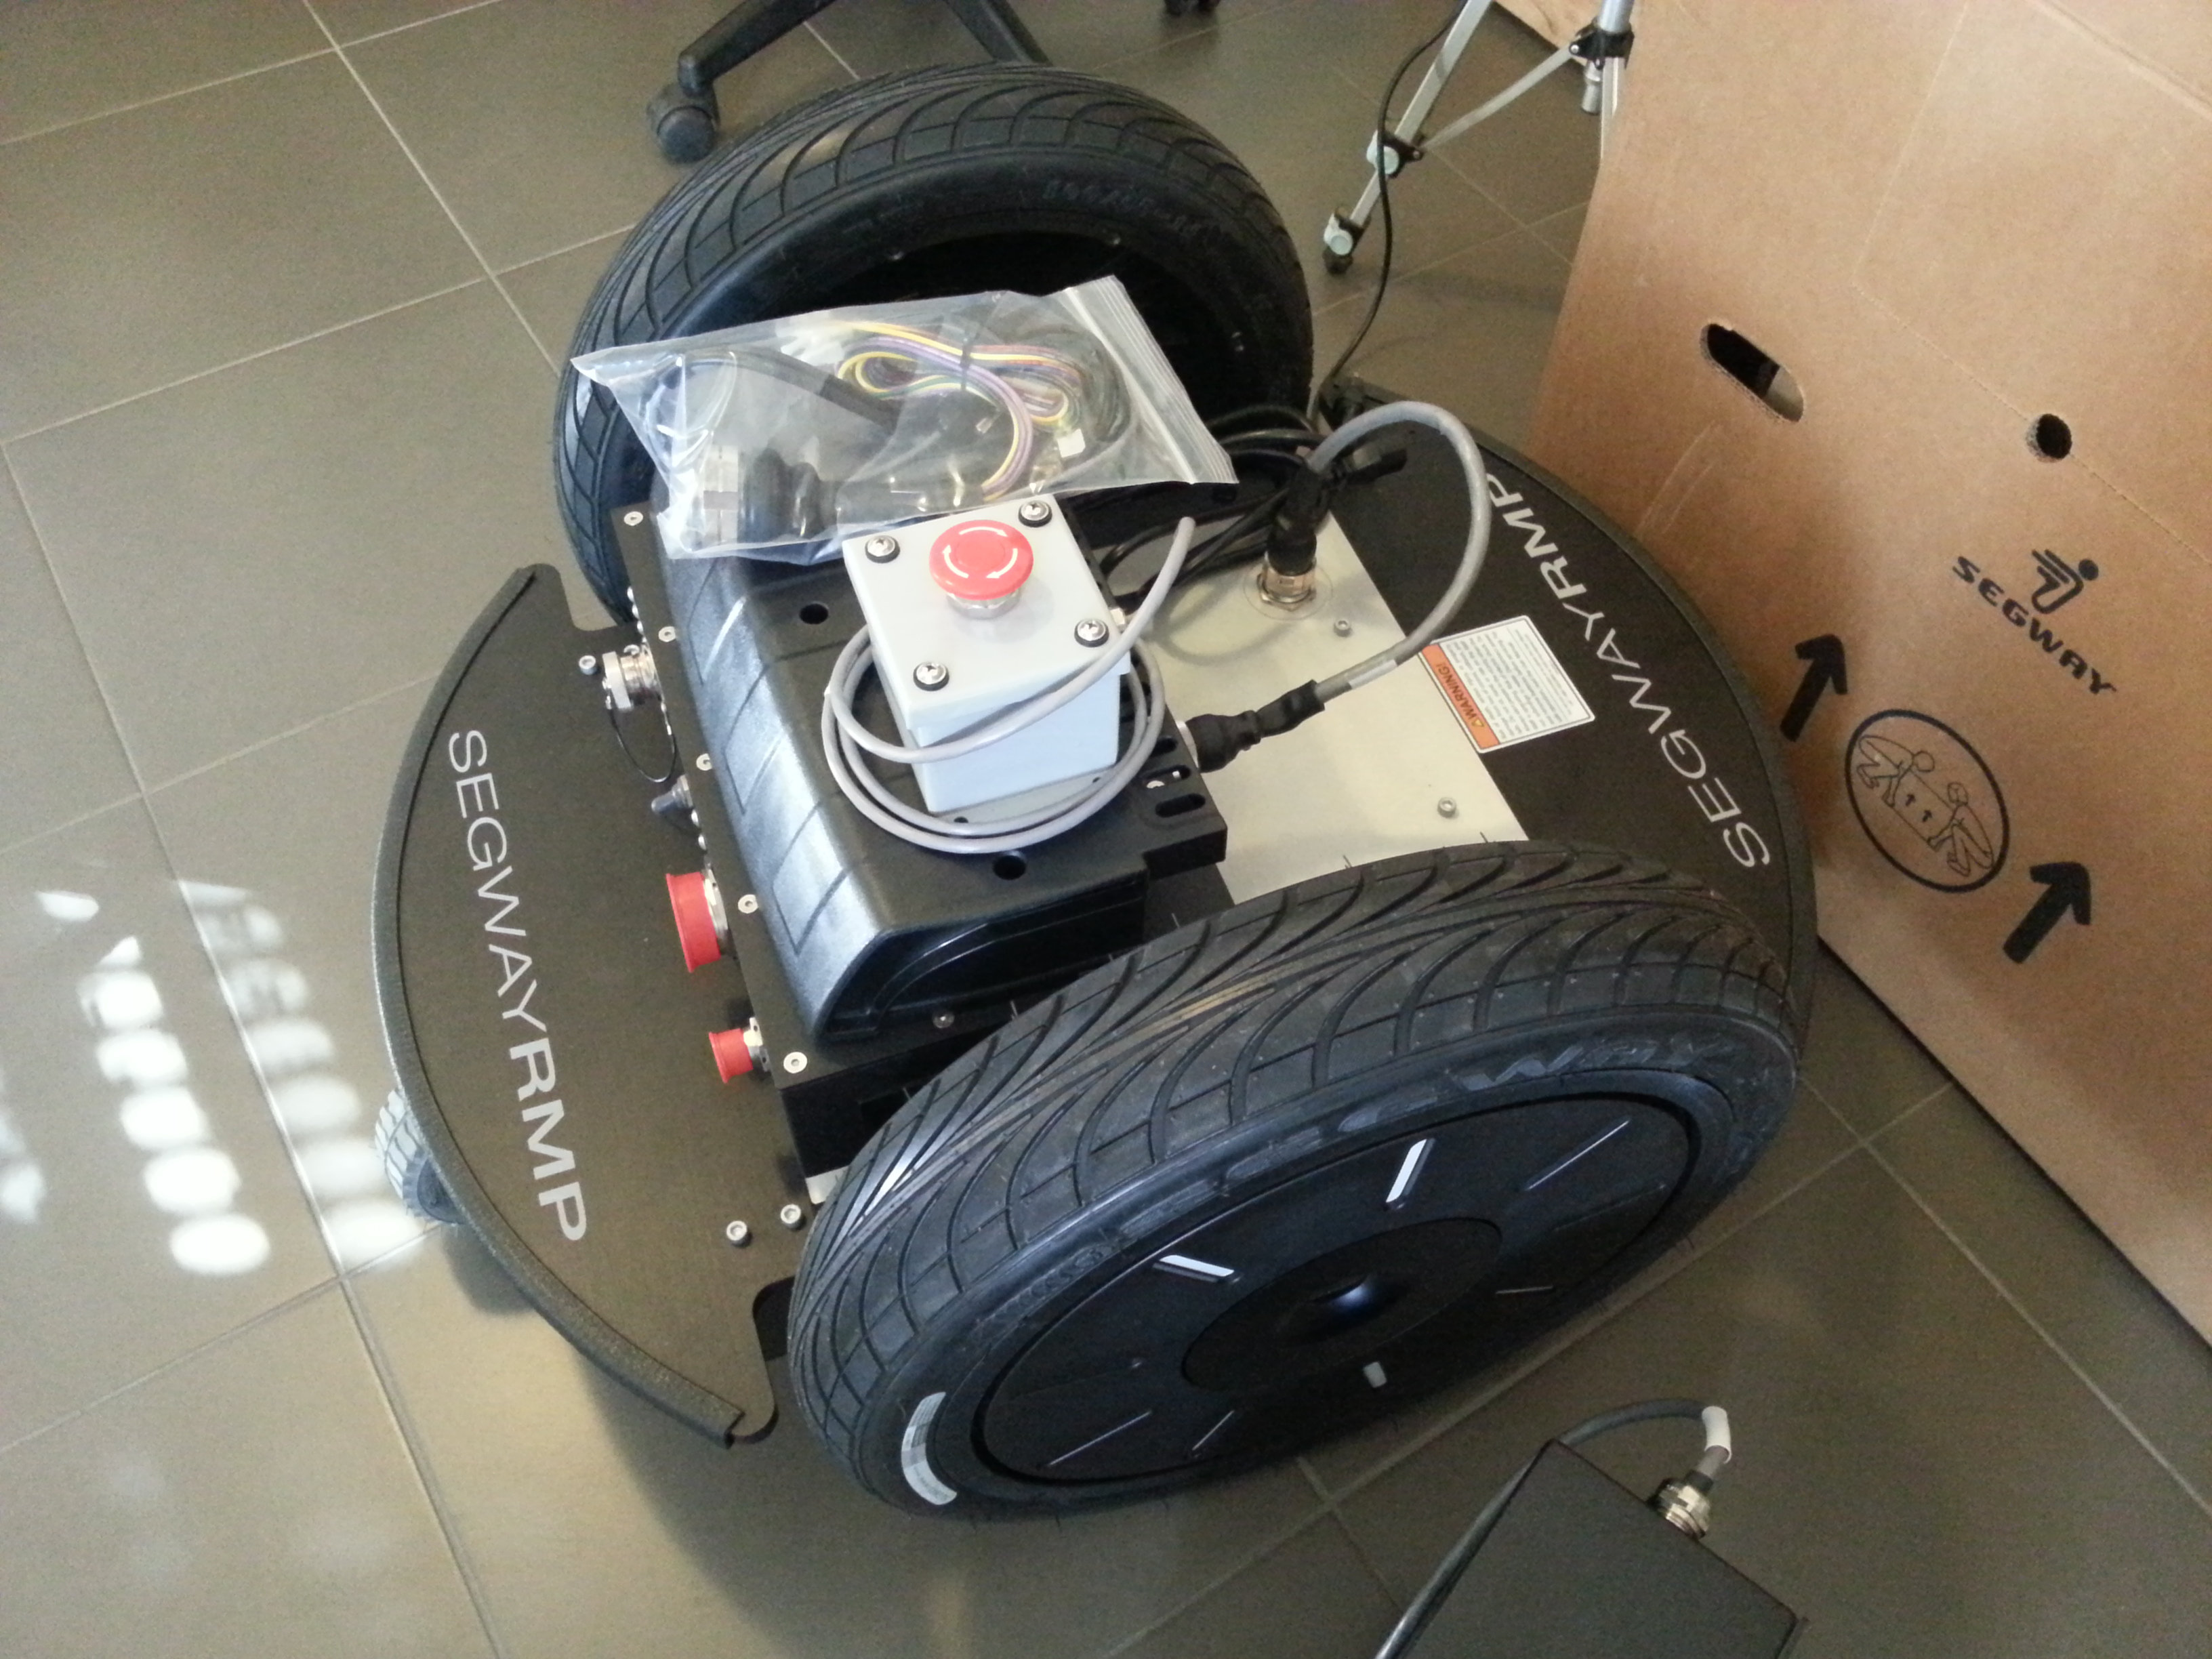
\includegraphics[height=5cm]{fig/segway_rmp210.jpg}
\end{center}

brief description of main technical characteristics...



{\bf Laser range finders - Front: UTM-30-LX, Back: Hokuyo URG-04LX-UG01}

PHOTO

DESCRIPTION



{\bf Cameras: 2 ASUS Xtion pro Live, Logitech C920}




Speakers:

Microphone: Microphone RODE NTG-2  (directional microphone) ...

PC laptop: HP EliteBook 820 G2

Tablet: Microsoft Surface Pro 2

SBC: 3 Odroid C1

Network switch for internal communication and external wireless communication




\subsection{Device Connections}

Robot, 2 Laser, 3 Cameras -USB- 2 Bananas

3 Odroid  -Ethernet- Net Switch

Laptop, Tablet -Ethernet- Net Switch

Microphone -USB- Tablet

Speakers -audio jack- Tablet

External devices -Wireless- Net switch



\subsection{Device drivers}

thin\_drivers ...






